%--------------------------------------------------------------------------
%	PACKAGES AND OTHER DOCUMENT CONFIGURATIONS
%--------------------------------------------------------------------------
\documentclass[12pt,a4paper]{article}
\usepackage[utf8]{inputenc}
\usepackage[english]{babel}
\usepackage[T1]{fontenc}
\usepackage{amsmath}
\usepackage{amsfonts}
\usepackage{amssymb}
\usepackage{graphicx}
\usepackage{lmodern}
\usepackage[left=3cm,right=3cm,top=2.5cm,bottom=2.5cm]{geometry}

\usepackage{fancyhdr} % Required for custom headers
\usepackage{lastpage} % Required to determine the last page for the footer
\usepackage{extramarks} % Required for headers and footers
\usepackage[usenames,dvipsnames]{color} % Required for custom colors
\usepackage{graphicx} % Required to insert images
\usepackage{caption}
\usepackage{subcaption}
\usepackage{listings} % Required for insertion of code
%\usepackage{courier} % Required for the courier font
\usepackage{verbatim}
\usepackage{multirow}
\usepackage{eurosym}
\usepackage{url}
\usepackage{hyperref}
\usepackage{color}

\usepackage{todonotes}

\lstset{
	language=bash,
	tabsize=4,
	rulecolor=,
    basicstyle=\scriptsize,
    upquote=true,
    aboveskip={1.5\baselineskip},
    columns=fixed,
    showstringspaces=false,
    extendedchars=true,
    breaklines=true,
    %prebreak = \raisebox{0ex}[0ex][0ex]{\ensuremath{\hookleftarrow}},
    frame=single,
    showtabs=false,
    showspaces=false,
    showstringspaces=false,
    numbers=left,
    stepnumber=0
}

\setlength\parindent{0pt} % Removes all indentation from paragraphs

% sections in Alph
\renewcommand{\thesection}{\Roman{section}}

\begin{document}
	
%--------------------------------------------------------------------------
%	TITLE PAGE
%--------------------------------------------------------------------------
\begin{titlepage}
\newcommand{\HRule}{\rule{\linewidth}{0.5mm}} % Defines a new command for the horizontal lines, change thickness here
\centering % Center everything on the page
 
%	HEADING SECTIONS
\begin{figure}[!h]
	\begin{center}
	
\includegraphics[height=4cm]{liu.jpg}
	\end{center}
\end{figure}

%\null
%\vspace{1cm}
%\textsc{\Large Linköping University}\\[1cm] % Name of your university/college
\textsc{\large Department of Computer and Information Science}\\[0.5cm] % Major heading such as course name
\textsc{\large TDTS06 Computer Networks}\\[2.5cm] % Minor heading such as course title

%	TITLE SECTION

\HRule \\[0.4cm]
{ \LARGE \bfseries Distance Vector Routing\\[0.4cm] % Title of your document
\Large \bfseries Report} \\[0.4cm]

\HRule \\[1.5cm]


%	AUTHOR SECTION

\large
\begin{centering}
Group C/D 13 \\[0.2cm]
\end{centering}
{\begin{tabular}{lll}
\textsc{Chvátal} & Martin & march011@student.liu.se\\
\textsc{Peschke} & Lena & lenpe782@student.liu.se\\
\end{tabular}}
\\[1.5cm]

\normalsize
Teaching assistant :\\[0.2cm]
{\begin{tabular}{ll}
\textsc{Schmidt} Johannes & johannes.schmidt@liu.se \\
\end{tabular}}
\\[2cm]

%	DATE SECTION
\vfill
{\normalsize \today} % Date, change the \today to a set date if you want to be precise

\newpage

\end{titlepage}

%--------------------------------------------------------------------------
%	TABLE OF CONTENTS
%--------------------------------------------------------------------------

%\pagenumbering{gobble}
%\clearpage
%\thispagestyle{empty}
%\tableofcontents
%\clearpage
%\pagenumbering{arabic}

%--------------------------------------------------------------------------
%	CONTENT
%--------------------------------------------------------------------------
  
% i
\section{How distance vector routing works}
\paragraph{In general}
Distance vector routing uses a decentralized routing algorithm to find the least-cost path between routers in a network.
The distance vector routing algorithm considers a network as an undirected graph of routers, represented as nodes, and links, represented as edges. It is iterative, asynchronous and distributed \cite[p.~371]{cn}. It makes use of the Bellman-Ford equation:
\begin{equation}
d_x(y) = \min_v\{c(x,v) + d_v(y)\}
\label{eq:bf}
\end{equation}
The equation states that the cost of the least-cost path from node $x$ to $y$, $d_x(y)$, is the minimum of the sum of the cost to get from $x$ to a neighbor $v$ and the cost of the least-cost path from $v$ to $y$.

The algorithm works by making the nodes exchange distance vectors.
To make use of the equation, each node needs to know about all of the other nodes in the network and the cost to its direct neighbors. Let's walk through the algorithm step by step.

\begin{enumerate}
\item Initially, each node knows the cost to its direct neighbors. It sends its distance vector to its neighbors.

\item Upon receiving an update (link cost change or new distance vector from a neighbor), a node recomputes its distance vector using the Bellman-Ford equation~(\ref{eq:bf}). If there is a change, it sends its own new vector to the all the neighbors.

\item ``The process of receiving updated distance vectors from neighbors, recomputing routing table entries, and informing neighbors of changed costs of the least-cost path to a destination continues until no update messages are sent.''~\cite[p.~375]{cn}
\end{enumerate}

After step 3, the estimated costs have converged to the actual least-costs.

% ii
\section{How we tested the algorithm}
\todo[inline]{wait for the code}

% iii
\section{Poisoned reverse}
% explain what it is
When a link cost in the network increases, a count-to-infinity problem can occur. A packet can then be caught in a routing loop until the nodes have figured out the shortest path, which can take a while (as many iterations as the difference between the previous and the new least-cost). Poisoned reverse is an addition to the DVR algorithm which helps avoiding this situation. If a node $x$ routes through $y$ in order to get to $z$, $x$ lies to $y$ about its distance to $z$, so that an increase in the cost link between $y$ and $z$ results in an convergent update that takes only two iterations. 

\paragraph{Where it fails}
% example topology
Poisonous reverse fails if a count-to-infinity problem triggers a loop of three or more nodes \cite[p.~378]{cn}.

Let us consider a network of 4 routers, $A$, $B$, $C$ and $D$. The network is represented below in Figure~\ref{fig:fail}. For this example, we will analyse partial routing tables which show the different path costs from one node to all of the others in the network. The example is inspired by~\cite{berkeley}.

\begin{description}
\item[Initial situation] Initially, all links have a cost of 1. The routing tables for nodes $A$ and $B$ are represented in Tables~\ref{tab:inita} and~\ref{tab:initb}. The least-cost routes to the different nodes in the network are emphasised in blue. In Table~\ref{tab:inita}, any path through $D$ has an $\infty$ cost because $A$ and $D$ are not connected, and to go via $D$, there is always a back-and-forth. In Table~\ref{tab:initb}, the two $\infty$ result directly from poisonous reverse, since $A$ and $C$ route through $B$ to get to $D$.

\item[Step 1] The cost of the link between $B$ and $D$ changes from 1 to 50. $B$ and $D$ get the information and update their tables. $B$'s new routing table is given in Table~\ref{tab:step1}.

\item[Step 2] $B$ sends its updated table across the network. $A$ gets the information and updates its own table, given in Table~\ref{tab:step2}. $A$ believes there is a path via $C$, not knowing that $C$ also routes via $B$.

\item[Step 3] $B$ gets the update from $A$ and updates its own table, as can be seen in Table~\ref{tab:step3}. As $A$ advertises a route through $C$, $B$ now also thinks there is a path with a lesser cost than 50 to $D$. From here on, we can see that a count-to-infinity situation occurs and will not stop until the actual cost is detected, requiring 47 more updates between $A$ and $B$ (leaving $C$ out).
\end{description}

\begin{figure}[!ht]
\centering
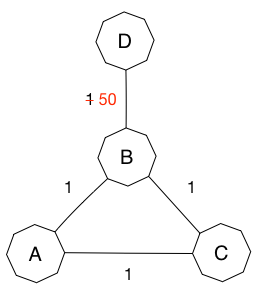
\includegraphics[width=0.35\textwidth]{Fail.png}
\caption{Example topology where poisoned reverse fails.}
\label{fig:fail}
\end{figure}

\begin{table}[!ht]
\begin{minipage}{0.5\textwidth}
\centering
\begin{tabular}{c|ccc}
	& \multicolumn{3}{c}{\textit{via}} 						\\
	&	B			&	C			&	D					\\
\hline
B	& 	\textcolor{Cyan}{1}	&	2			&	$\infty$	\\
C	&	2			&	\textcolor{Cyan}{1}	&	$\infty$	\\
D	&	\textcolor{Cyan}{2}	&	3			&	$\infty$	\\
\end{tabular}
\caption{$A$'s initial routing table}
\label{tab:inita}
\end{minipage}
\hfill
\begin{minipage}{0.5\textwidth}
\centering
\begin{tabular}{c|ccc}
	& \multicolumn{3}{c}{\textit{via}} 						\\
	&	A			&	C			&	D					\\
\hline
A	& 	\textcolor{Cyan}{1}	&	2			&	$\infty$	\\
C	&	2			&	\textcolor{Cyan}{1}	&	$\infty$	\\
D	&	$\infty$	&	$\infty$	&	\textcolor{Cyan}{1}	\\
\end{tabular}
\caption{$B$'s initial routing table}
\label{tab:initb}
\end{minipage}
\end{table}

\begin{table}[!ht]
\centering
\begin{tabular}{c|ccc}
	& \multicolumn{3}{c}{\textit{via}} 						\\
	&	A			&	C			&	D					\\
\hline
A	& 	\textcolor{Cyan}{1}	&	2			&	$\infty$	\\
C	&	2			&	\textcolor{Cyan}{1}	&	$\infty$	\\
D	&	$\infty$	&	$\infty$	&	\textcolor{Cyan}{50}\\
\end{tabular}
\caption{$B$'s routing table after step 1}
\label{tab:step1}
\end{table}

\begin{table}[!ht]
\centering
\begin{tabular}{c|ccc}
	& \multicolumn{3}{c}{\textit{via}} 						\\
	&	B			&	C			&	D					\\
\hline
B	& 	\textcolor{Cyan}{1}	&	2			&	$\infty$	\\
C	&	2			&	\textcolor{Cyan}{1}	&	$\infty$	\\
D	&	51			&	\textcolor{Cyan}{3}	&	$\infty$	\\
\end{tabular}
\caption{$A$'s routing table after step 2}
\label{tab:step2}
\end{table}

\begin{table}[!ht]
\centering
\begin{tabular}{c|ccc}
	& \multicolumn{3}{c}{\textit{via}} 						\\
	&	A			&	C			&	D					\\
\hline
A	& 	\textcolor{Cyan}{1}	&	2			&	$\infty$	\\
C	&	2			&	\textcolor{Cyan}{1}	&	$\infty$	\\
D	&	\textcolor{Cyan}{4}	&	$\infty$	&	50			\\
\end{tabular}
\caption{$B$'s routing table after step 3}
\label{tab:step3}
\end{table}

\paragraph{Solutions}
In practise, the Routing Information Protocol (RIP) uses DVR with poisoned reverse where infinity is 16 hops. This does not avoid the count-to-infinity problem, but limits the damage by stopping updates after it reaches `ìnfinity''.
In addition, \textit{hold-down timers} can be used: if a route becomes unusable, it is kept in the tables with an infinity value for a certain amount of time. If an update advertises a better or equally good route, it is replaced. On the other hand, if the update indicates a worse cost, it is ignored. 

Another solution (which actually solves the problem) is using \textit{path vectors}: in addition to the distance vectors, we can keep a record of the path, i. e. the nodes traversed to obtain the cost. When a link cost increases or a link disappears from the network, a node can check if the path is still valid by looking it up. This is used in BGP~\cite{mit}.

\bibliographystyle{alpha}
\bibliography{biblio}
\nocite{*}
    
\end{document}